\section{Soluci\'on Propuesta}

\begin{frame}{Soluci\'on Propuesta (1/5)}
\framesubtitle{TamTam Edit}

\begin{figure}[H]
\centering
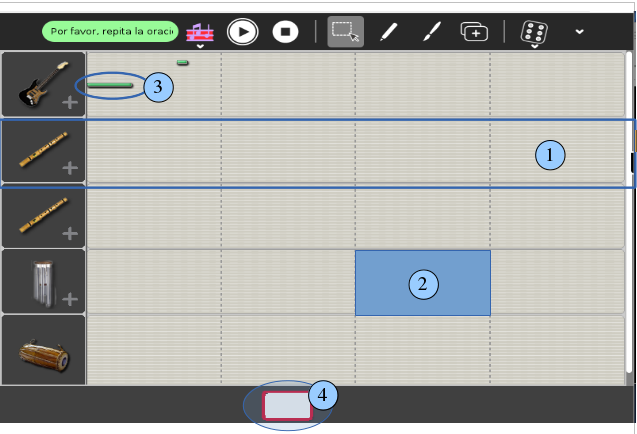
\includegraphics[width=0.8\textwidth]{./graphics/ui-tamtam-edit.png}
\caption{Interfaz de \emph{Tamtam Edit} y sus secciones principales.}
\label{figure:ui-tamtam}
\end{figure}

\end{frame}

\begin{frame}{Soluci\'on Propuesta (2/5)}
\framesubtitle{TamTam Listens}

\only<1>{\begin{figure}[H] 
\centering
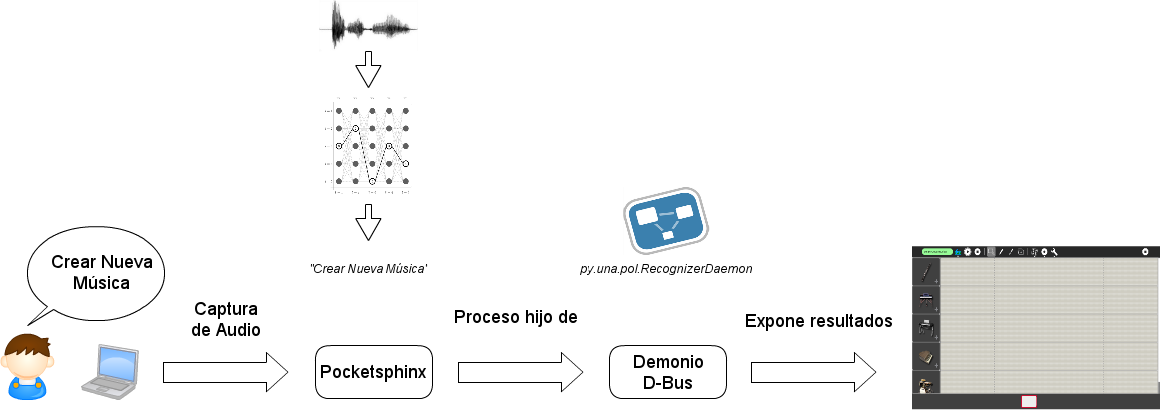
\includegraphics[width=1.0\textwidth]{./graphics/tamtam-proceso-4.png}
\caption{Arquitectura de Tamtam Listens}
\label{figure:tamtam-listens-proceso-4}
\end{figure}}

\only<2>{\begin{figure}[H] 
\centering
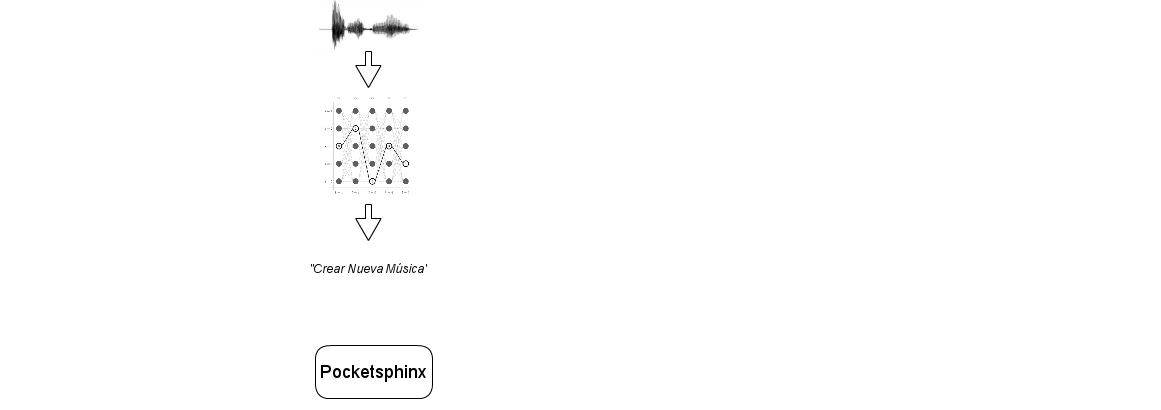
\includegraphics[width=1.0\textwidth]{./graphics/tamtam-proceso-1.png}
\caption{Arquitectura de Tamtam Listens. Motor de Reconocimiento}
\label{figure:tamtam-listens-proceso-1}
\end{figure}}

\only<3>{\begin{figure}[H] 
\centering
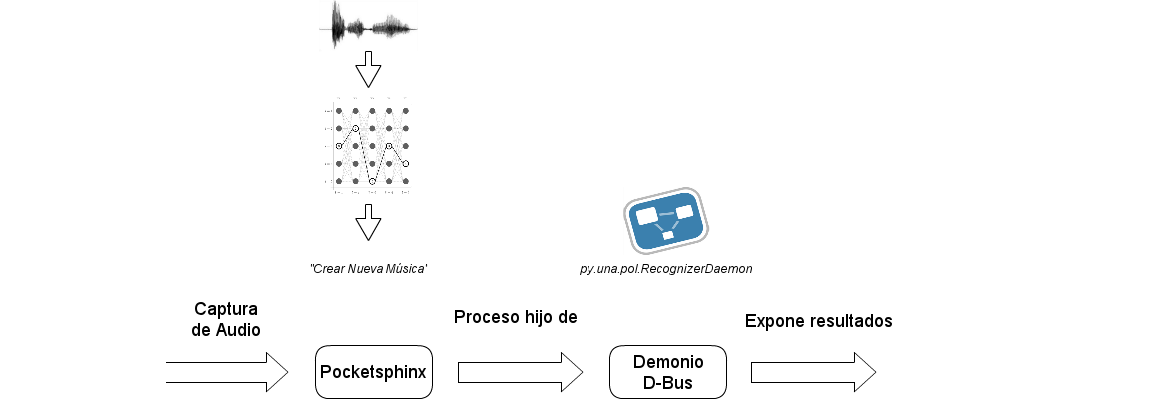
\includegraphics[width=1.0\textwidth]{./graphics/tamtam-proceso-3.png}
\caption{Arquitectura de Tamtam Listens. Servicio de reconocimiento}
\label{figure:tamtam-listens-proceso-3}
\end{figure}}

\only<4>{\begin{figure}[H] 
\centering
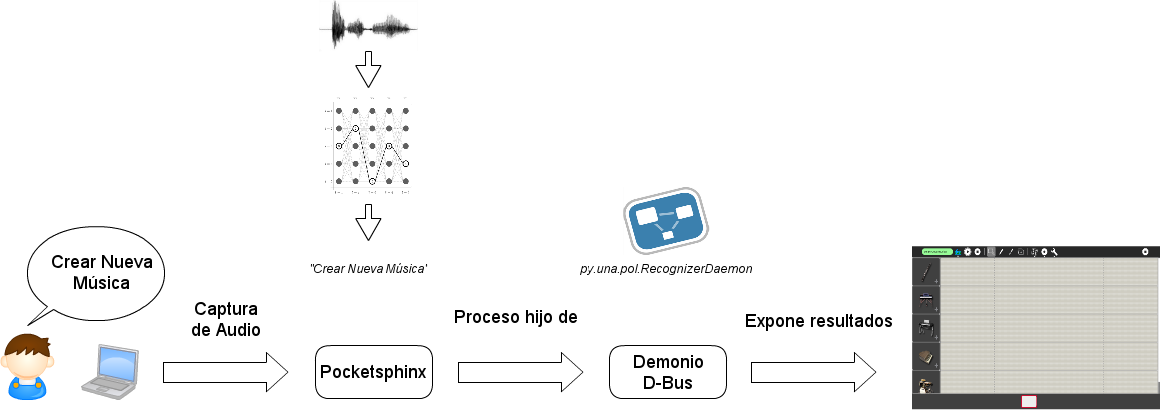
\includegraphics[width=1.0\textwidth]{./graphics/tamtam-proceso-4.png}
\caption{Arquitectura de Tamtam Listens}
\label{figure:tamtam-listens-proceso-4}
\end{figure}}

\end{frame}

\begin{frame}{Soluci\'on Propuesta (3/5)}
\framesubtitle{TamTam Listens}

\only<1>{\begin{figure}[H] 
\centering
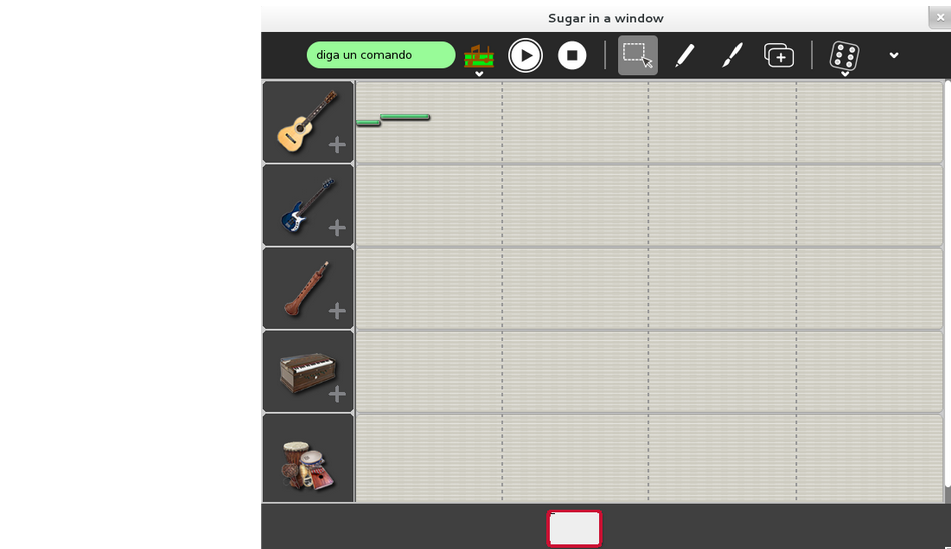
\includegraphics[width=1.0\textwidth]{./graphics/interaccion1.png}
\caption{Ejemplo de interacci\'on}
\label{figure:tamtam-listens-interaccion}
\end{figure}}

\only<2>{\begin{figure}[H] 
\centering
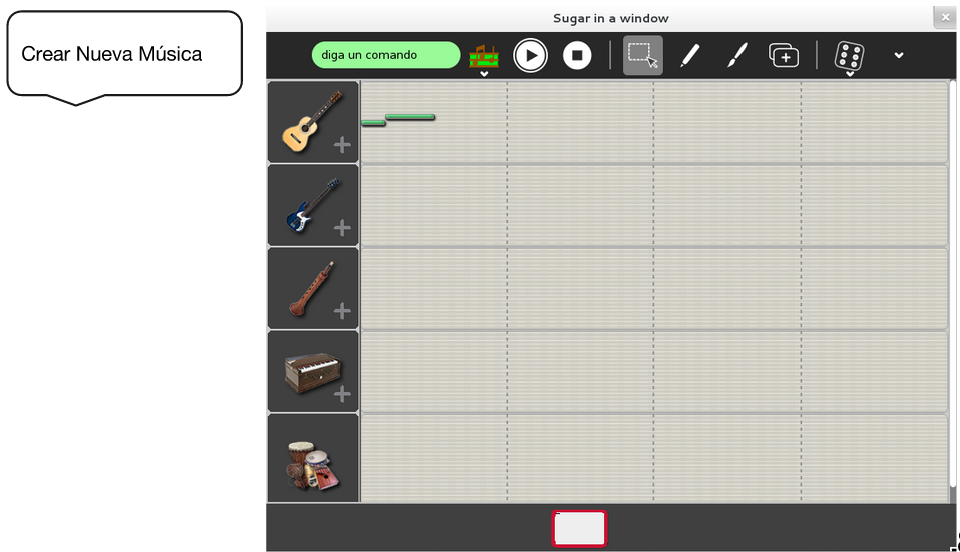
\includegraphics[width=1.0\textwidth]{./graphics/interaccion2.png}
\caption{Ejemplo de interacci\'on}
\label{figure:tamtam-listens-interaccion}
\end{figure}}

\only<3>{\begin{figure}[H] 
\centering
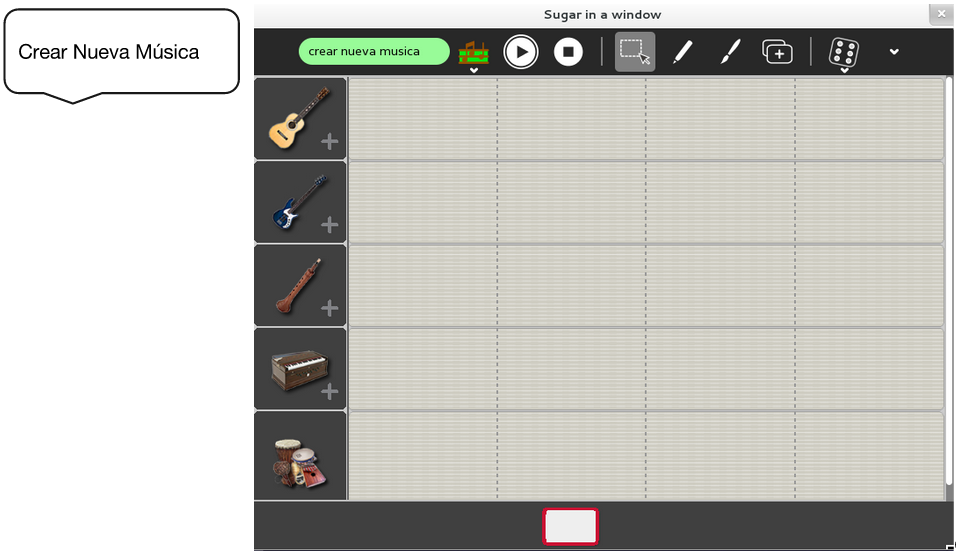
\includegraphics[width=1.0\textwidth]{./graphics/interaccion3.png}
\caption{Ejemplo de interacci\'on}
\label{figure:tamtam-listens-interaccion}
\end{figure}}

\only<4>{\begin{figure}[H] 
\centering
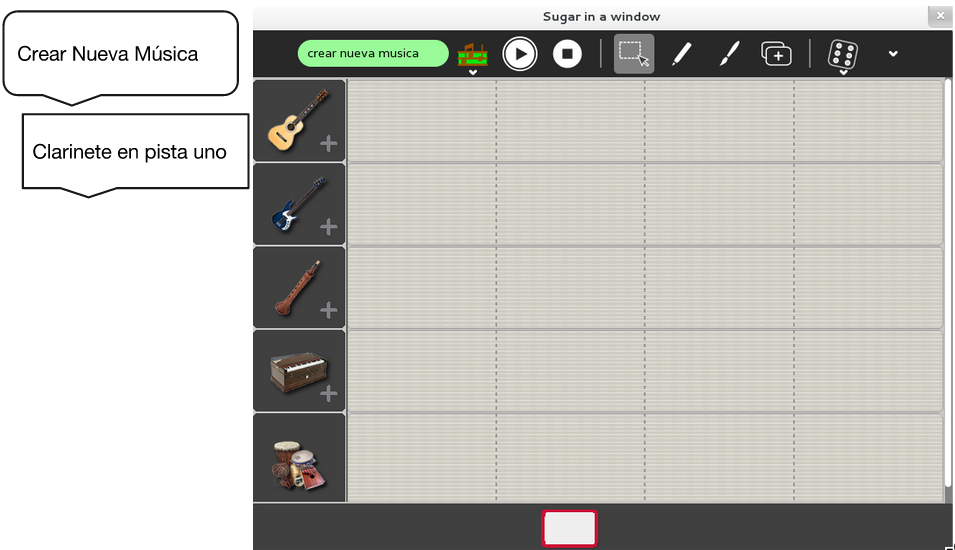
\includegraphics[width=1.0\textwidth]{./graphics/interaccion4.png}
\caption{Ejemplo de interacci\'on}
\label{figure:tamtam-listens-interaccion}
\end{figure}}

\only<5>{\begin{figure}[H] 
\centering
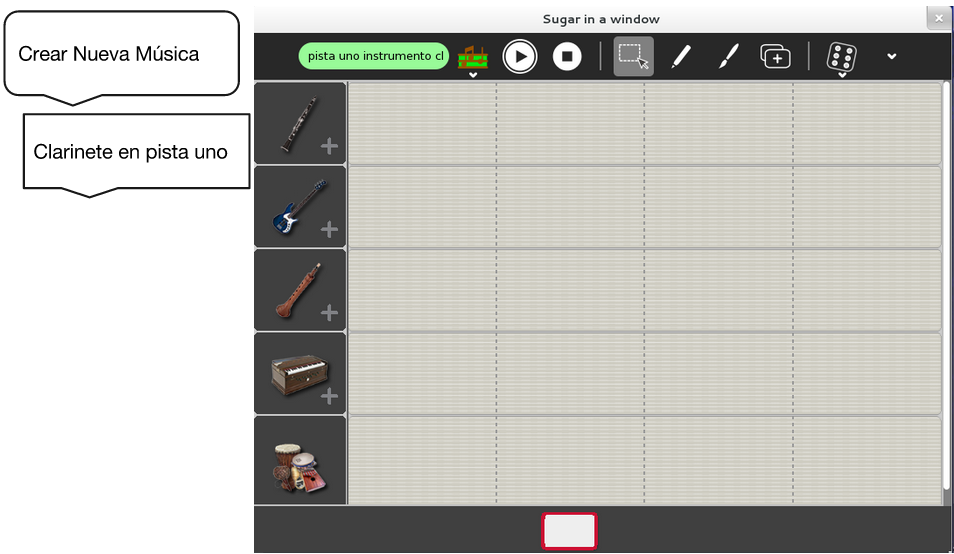
\includegraphics[width=1.0\textwidth]{./graphics/interaccion5.png}
\caption{Ejemplo de interacci\'on}
\label{figure:tamtam-listens-interaccion}
\end{figure}}


\only<6>{\begin{figure}[H] 
\centering
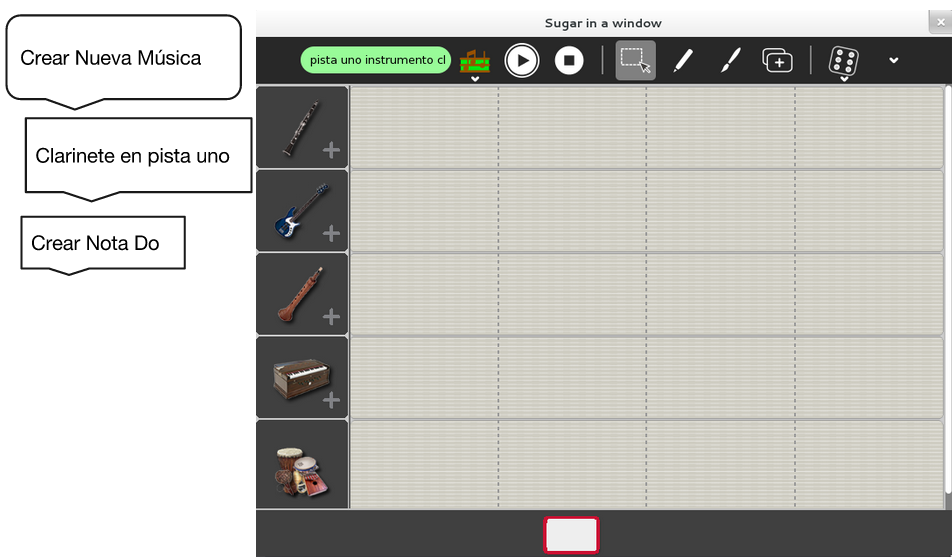
\includegraphics[width=1.0\textwidth]{./graphics/interaccion6.png}
\caption{Ejemplo de interacci\'on}
\label{figure:tamtam-listens-interaccion}
\end{figure}}

\only<7>{\begin{figure}[H] 
\centering
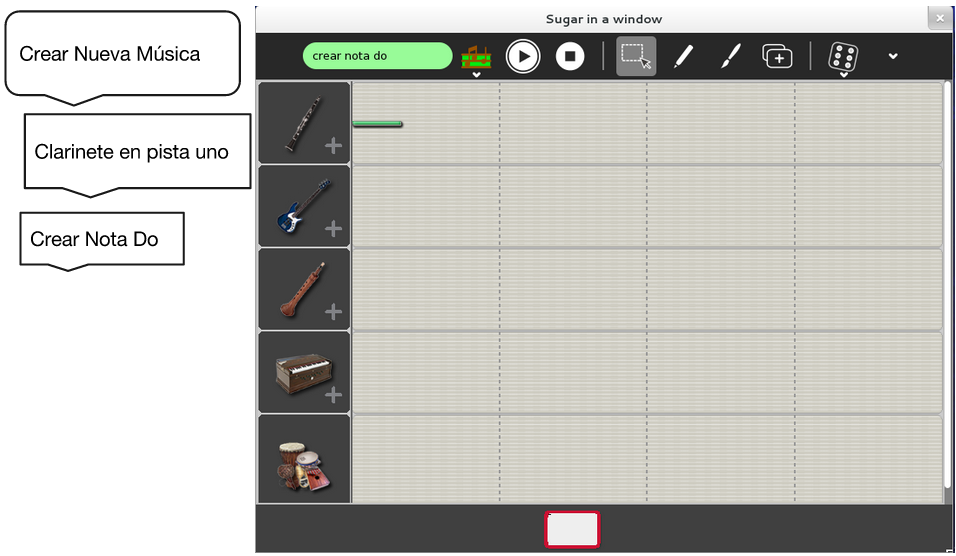
\includegraphics[width=1.0\textwidth]{./graphics/interaccion7.png}
\caption{Ejemplo de interacci\'on}
\label{figure:tamtam-listens-interaccion}
\end{figure}}

\only<8>{\begin{figure}[H] 
\centering
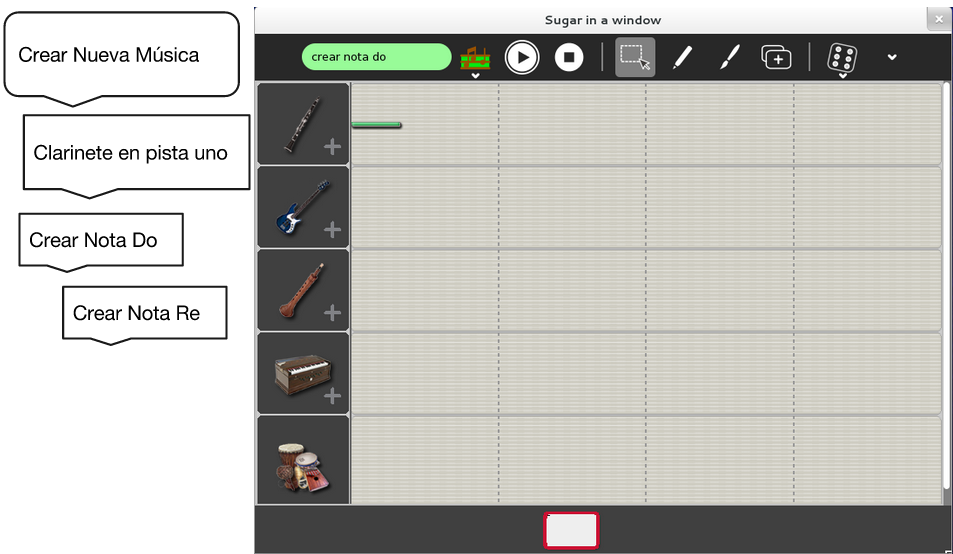
\includegraphics[width=1.0\textwidth]{./graphics/interaccion8.png}
\caption{Ejemplo de interacci\'on}
\label{figure:tamtam-listens-interaccion}
\end{figure}}

\only<9>{\begin{figure}[H] 
\centering
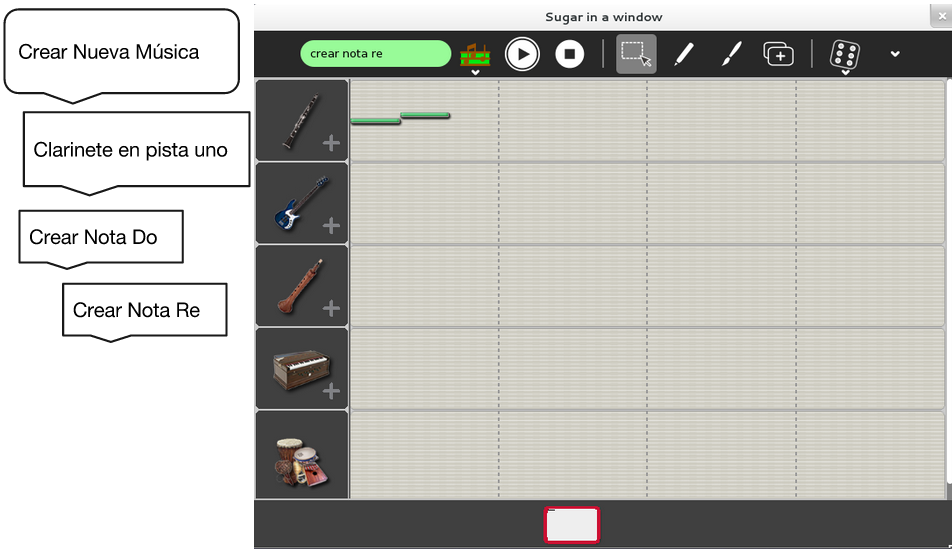
\includegraphics[width=1.0\textwidth]{./graphics/interaccion9.png}
\caption{Ejemplo de interacci\'on}
\label{figure:tamtam-listens-interaccion}
\end{figure}}

\only<10>{\begin{figure}[H] 
\centering
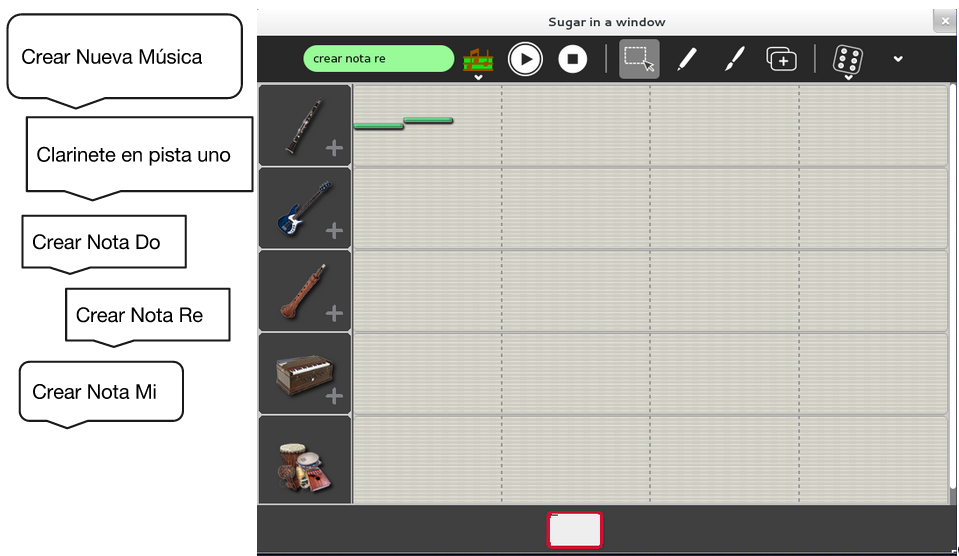
\includegraphics[width=1.0\textwidth]{./graphics/interaccion10.png}
\caption{Ejemplo de interacci\'on}
\label{figure:tamtam-listens-interaccion}
\end{figure}}

\only<11>{\begin{figure}[H] 
\centering
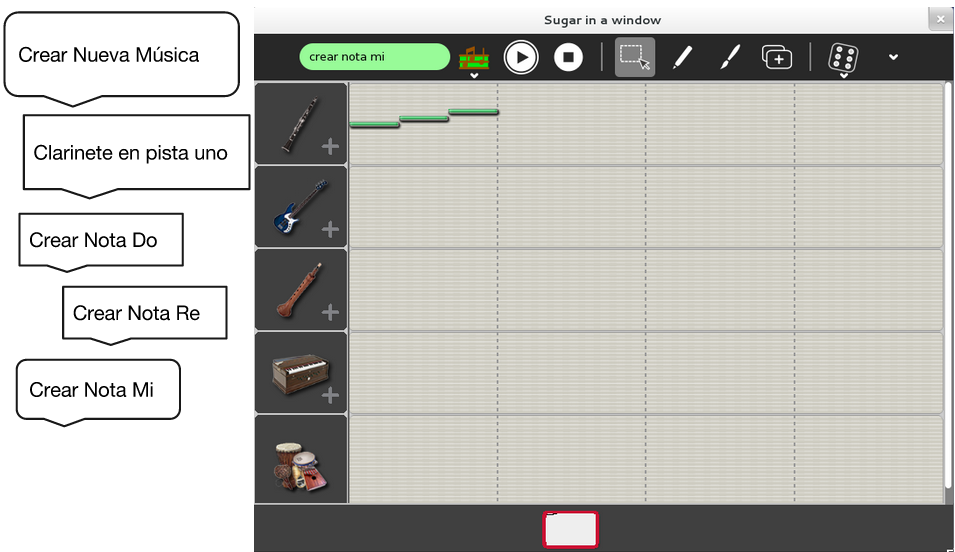
\includegraphics[width=1.0\textwidth]{./graphics/interaccion11.png}
\caption{Ejemplo de interacci\'on}
\label{figure:tamtam-listens-interaccion}
\end{figure}}

\only<12>{\begin{figure}[H] 
\centering
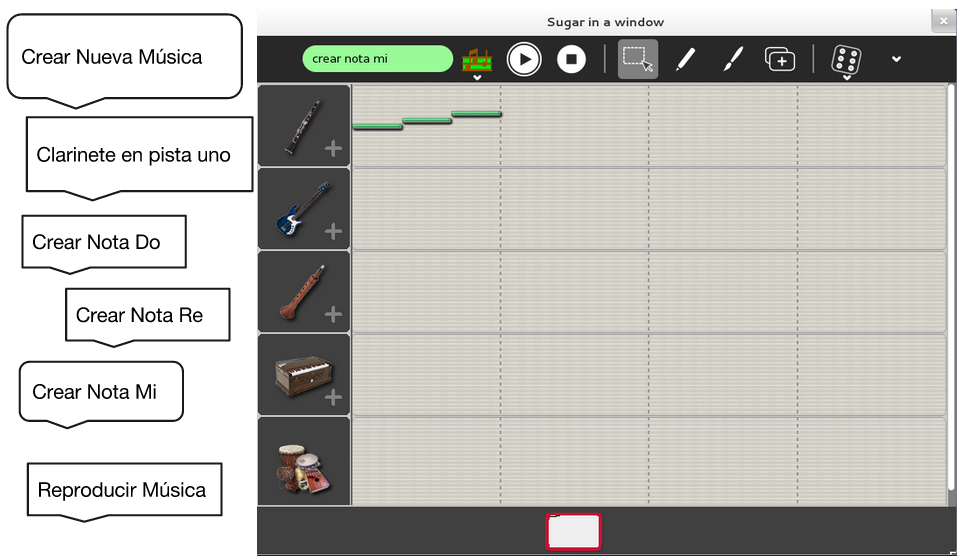
\includegraphics[width=1.0\textwidth]{./graphics/interaccion12.png}
\caption{Ejemplo de interacci\'on}
\label{figure:tamtam-listens-interaccion}
\end{figure}}

\only<13>{\begin{figure}[H] 
\centering
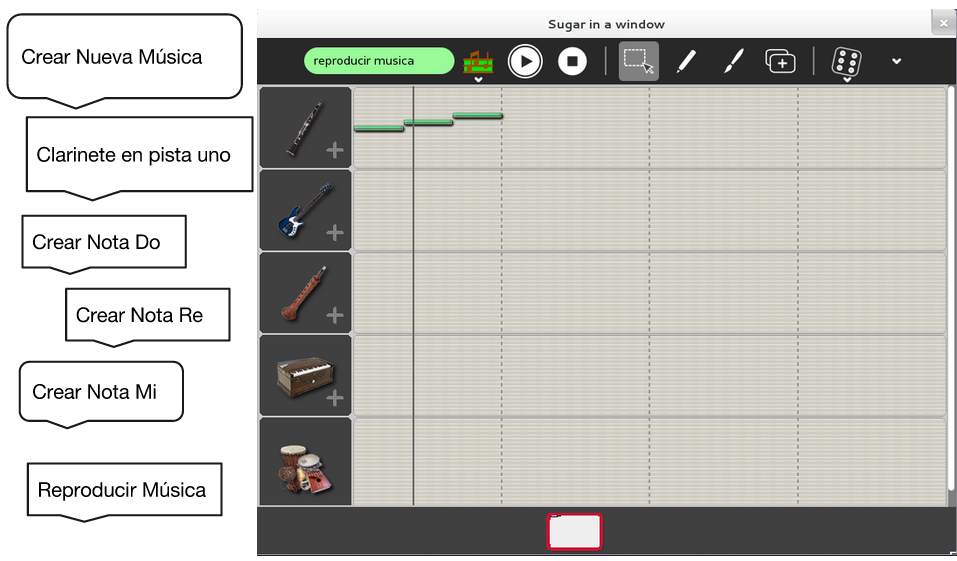
\includegraphics[width=1.0\textwidth]{./graphics/interaccion13.png}
\caption{Ejemplo de interacci\'on}
\label{figure:tamtam-listens-interaccion}
\end{figure}}

\end{frame}


\begin{frame}[fragile]{Soluci\'on Propuesta (4/5)}
\framesubtitle{Modelo de Lenguaje}
\begin{figure}[H]
\lstset{basicstyle=\ttfamily\scriptsize}
\begin{lstlisting}
#JSGF V1.0;
grammar tamtam;

public <tamtam-listens> = <comando> | <pagina> | <pista-a>  |
                          <pista-b>  | <seleccionar-compas> | 
                          <crear-nota> | <seleccionar-nota> | 
                          <duplicar-nota> | <borrar-nota>   | 
                          <volumen> | <tempo> | <loop>      |
                          <configurar-nota> ;

<comando>  = REPRODUCIR MUSICA  | PAUSAR MUSICA   |
             PARAR MUSICA | GENERAR MUSICA        | 
             CREAR NUEVA MUSICA | EXPORTAR MUSICA | 
             SALIR DE TAMTAM;
<pagina>   = ( CREAR NUEVA | DUPLICAR | LIMPIAR ) 
              PARTITURA | PARTITURA <orden>;
<orden>    = ( ANTERIOR | SIGUIENTE );
<loop>     = (COMODIN)+;
\end{lstlisting}
\caption{Fragmento de la gram\'atica utilizada en \emph{Tamtam Listens}.}
\label{figure:fragmento-gram}
\end{figure} 
\end{frame}

\begin{frame}[fragile]{Soluci\'on Propuesta (5/5)}
\framesubtitle{Modelo Acústico}
\begin{itemize}
    \item Proyecto Voxforge
    \item Diccionario Fonético    
\end{itemize}

    \begin{figure}[H]
    \begin{lstlisting}
    REPRODUCIR RR E P R O D U S I R
    PAUSAR P A U S A R
    PARAR  P A R A R
    GENERAR  J E N E R A R
    PARTITURA P A R T I T U R A
    SIGUIENTE S I G I E N T E
    ANTERIOR A N T E R I O R
    \end{lstlisting}
    \caption{Fragmento del diccionario fon\'etico utilizado en \emph{Tamtam Listens}.}
    \label{figure:fragmento-dic}
\end{figure}

\end{frame}

